\section{Анализ существующих решений и формирование требований к проектируемому программному средству}
\label{sec:practice:itechart_characteristics}
    
В дипломном проекте поставлена задача создания веб-приложения для обмена файлами.
Данное приложение должно обеспечивать хранение, загрузку и скачивание файлов. Данное приложение следует проектировать и разрабатывать как систему, способную выполнять следующие функции:
\begin{itemize}
  \item обеспечивать хранение файлов;
  \item обеспечивать загрузку файлов;
  \item обеспечивать скачивание файлов.
\end{itemize}

\subsection{Требования к приложениям обмена файлами}
\label{sec:practice:itechart_characteristic:trebovania}
Требования, предъявляемые к приложениям для обмена файлами включат в себя:
\begin{itemize}
  \item требования к функциональным характеристикам;
  \item требования к надежности;
  \item настраиваемость;
  \item условия эксплуатации;
  \item требования к информационной и программной совместимости;
  \item требования к составу и параметрам технических средств;
  \item требования к документации.
\end{itemize}

Требования к функциональным характеристикам. При выборе между объектными и структурными методами следует использовать принцип концептуальной общности, который предполагает следование единой философии на всех этапах жиз-ненного цикла. Если предполагается использовать структурное программирование, то и на этапе анализа следует использовать структурный подход, а в случае использования объектно-ориентированных языков разработки - объектный анализ и объектное проектирование. При необходимости структурный и объектный подходы могут использоваться одновременно.

Требования к надежности – должны быть определены требования к обеспечению надежного функционирования: контроль входной и выходной информации, время и механизмы восстановления после программных и аппаратных отказов. 

Настраиваемость – программное обеспечение должно обладать адаптивными возможностями, то есть указывается, должны быть предусмотрены различные изменения в методах управления и бизнес процессах.

Условия эксплуатации описывают необходимое обслуживание, которое требуется для работы системы, например, создание резервных копий, реиндексерование баз и т. п., а также требования к квалификации персонала (пользователей и обслуживающего персонала).

Требования к составу и параметрам технических средств определяют необходимый состав технических средств с указанием их основных технических характеристик. Могут указываться требования к помещениям, в которых будет находиться оборудование. Также указываются требования к переносимости системы.

Требования к информационной и программной совместимости определяют требования к информационным структурам на входе и выходе, методам решения, исходным кодам, языкам программирования и программным средствам, используемым программным комплексом.

\subsection{Анализ существующих решений}
\label{sec:practice:itechart_characteristic:analiz}

\subsubsection{DepositFiles}~\\
\label{ssub:practice:itechart_characteristic:depositfiles}   


\begin{figure}[ht]
  \centering
  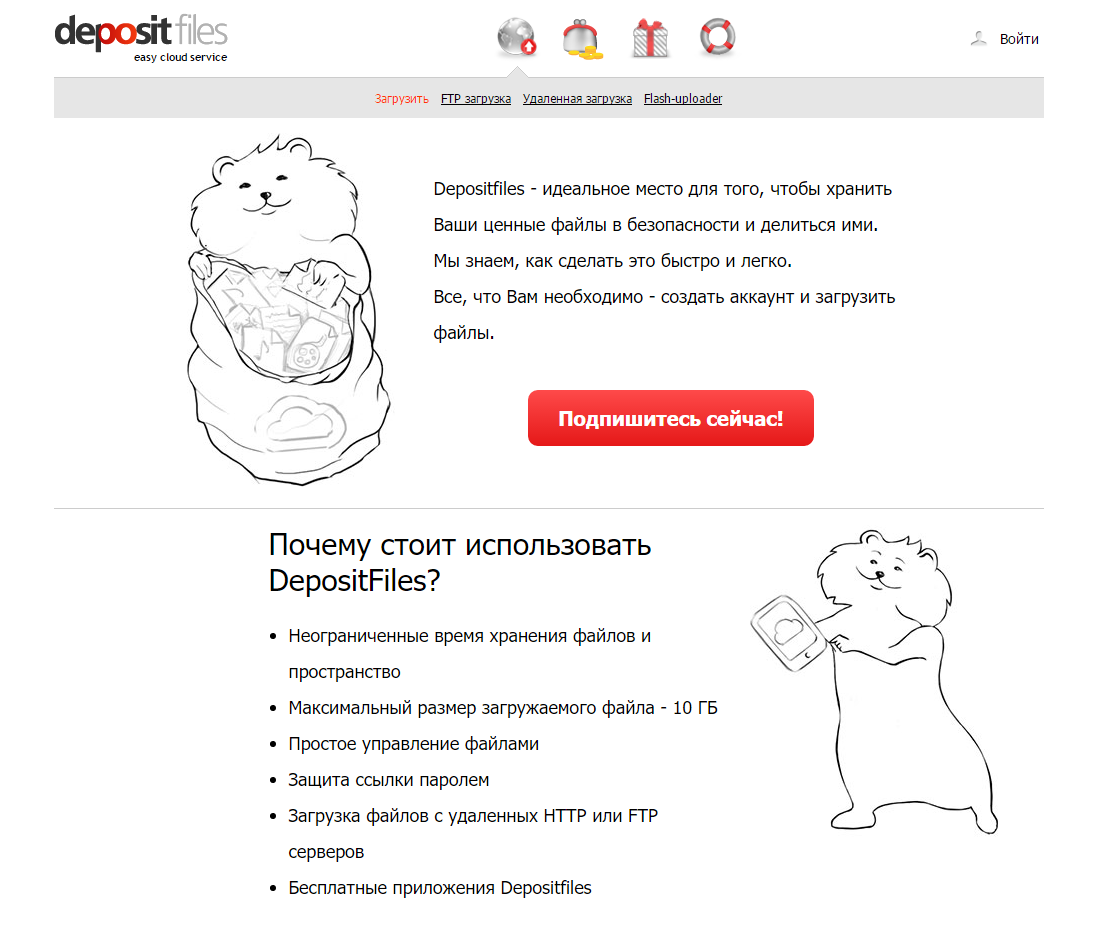
\includegraphics[scale=0.5]{deposit.png}  
    \caption{ Главная страница сервиса по обмену файлами DepositFiles. }
    \label{fig:deposit}
\end{figure}


Сервис «DepositFiles» (рисунок ~\ref{fig:deposit}) предоставляет функционал по загрузке и скачиванию файлов. Практически все элементы интерфейса собраны на главной странице. Кнопка «загрузить» позволяет пользователю с бесплатным аккаунтом загрузить до 50 файлов объёмом до 10 гигабайт. 

Возможности сервиса DepositFiles:
\begin{itemize}
  \item бесплатное хранение файлов на серверах неограниченное время;
  \item скачивание файлов с медленных серверов на сервис и их хранение;
  \item максимально возможный размер хранимого файла — 10 гигабайт;
  \item суммарный объем хранимых файлов неограничен;
  \item бесплатное программное обеспечение для работы с файлами;
  \item установка пароля на скачивание файла;
  \item удаление файла в удобное время;
  \item скачивание файла в удобное время. 
\end{itemize}

На страницах «гейт», «скачивания» и на странице «удаленные файлы» присутствует реклама. 
Сервис содержит полный набор атрибутов, необходимых для работы файлового хостинга и практически не содержит дополнительного функционала, не связанного с загрузкой пользовательских файлов. 
Таким образом, он представляет собой пример традиционного файлового хостинга и максимально упрощает навигацию пользователя за счёт простоты интерфейса.

\subsubsection{4shared}~\\
\label{ssub:practice:itechart_characteristic:4shared}

\begin{figure}[ht]
  \centering
  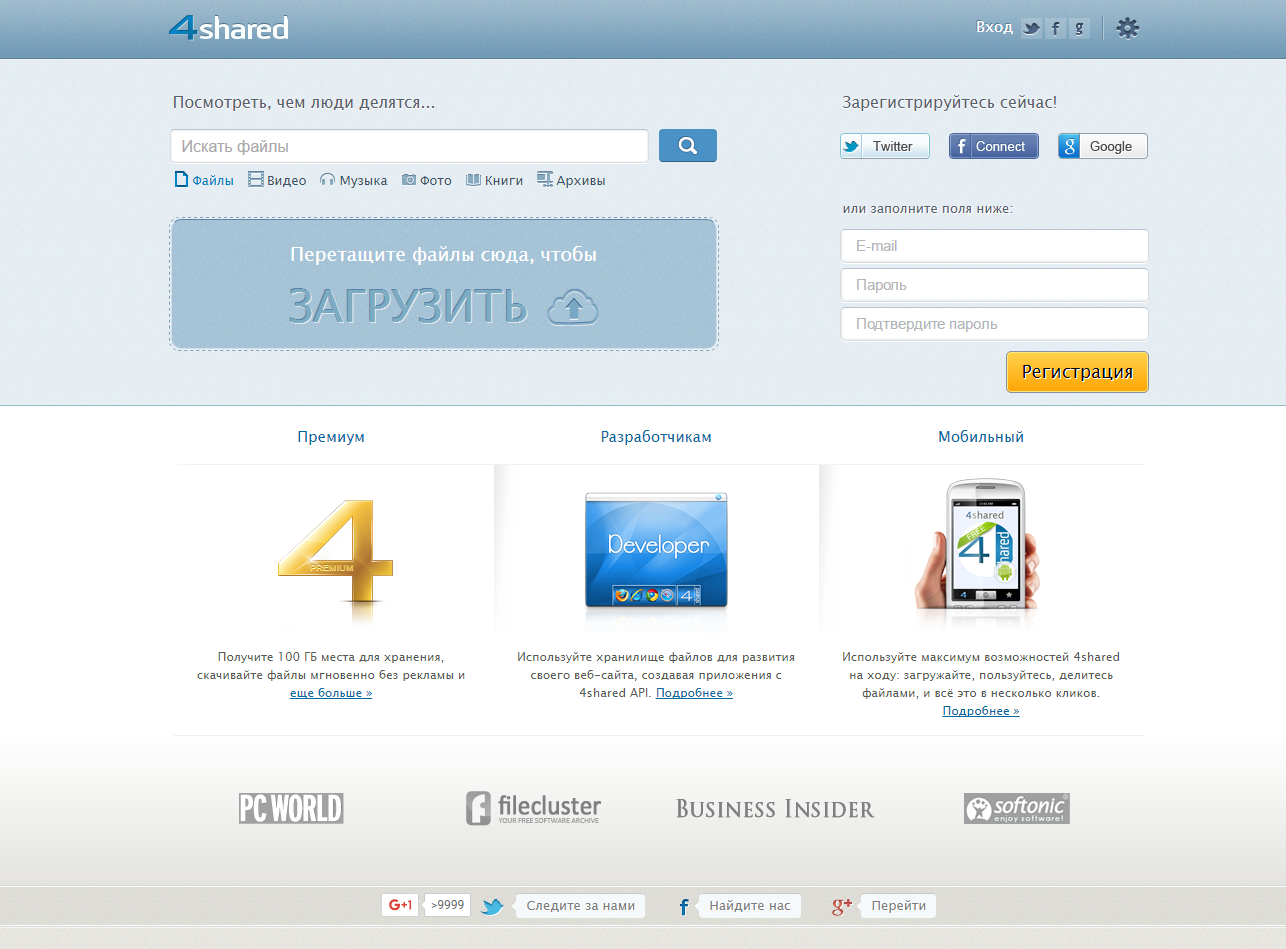
\includegraphics[scale=0.45]{4shared.png}  
    \caption{ Главная страница сервиса по обмену файлами 4shared. }
    \label{fig:4shared}
\end{figure}

Файловый хостинг «4shared.com» (рисунок ~\ref{fig:4shared}) предназначен для обмена файлами между пользователями, быстрого поиска необходимых файлов и просмотра содержимого файлов в реальном времени. За счет упорядочения и систематизации большого объема информации, необходимой для обеспечения работоспособности ресурса, достигается высокая скорость поиска и загрузки файлов.

Традиционно файловые хостинги не реализуют функционал, не связанный с обработкой пользовательских данных, однако «4shared.com» предоставляет некоторые возможности по настройке пользовательского интерфейса (фон, индикаторы, статистика).

Характерными особенностями системы является возможность просмотра содержимого интересующих пользователя файлов, возможность установить QR-коды для каждого файла, а также автоматическая архивация файла в процессе загрузки.

Сервис «4shared.com» позволяет загружать данные любого типа размером до 100 гигабайт, обладает объёмом виртуального диска до 100 гигабайт и способен восстанавливать удалённые файлы пользователей. Большая часть дополнительного функционала доступна только владельцам премиум-аккаунтов. 

Пользователю без премиум аккаунта доступен следующий функционал:
\begin{itemize}
  \item объём виртуального диска - 15 гигабайт;
  \item максимальный размер загружаемого файла - 2 гигабайта;
  \item количество субдоменов – 100;
  \item лимит трафика – 0;
  \item функция поиска;
  \item управление файлами онлайн;
  \item windows-интерфейс;
  \item совместимость с операционными системами Windows, Linux и Mac;
  \item многоуровневая система файлов;
  \item восстановление файлов.
\end{itemize}

Сервис имеет простой и удобный интерфейс, позволяющий быстро найти необходимые элементы управления и получить доступ к интересующему функционалу.  

\subsubsection{RGhost}~\\
\label{ssub:practice:itechart_characteristic:rghost}

\begin{figure}[ht]
  \centering
  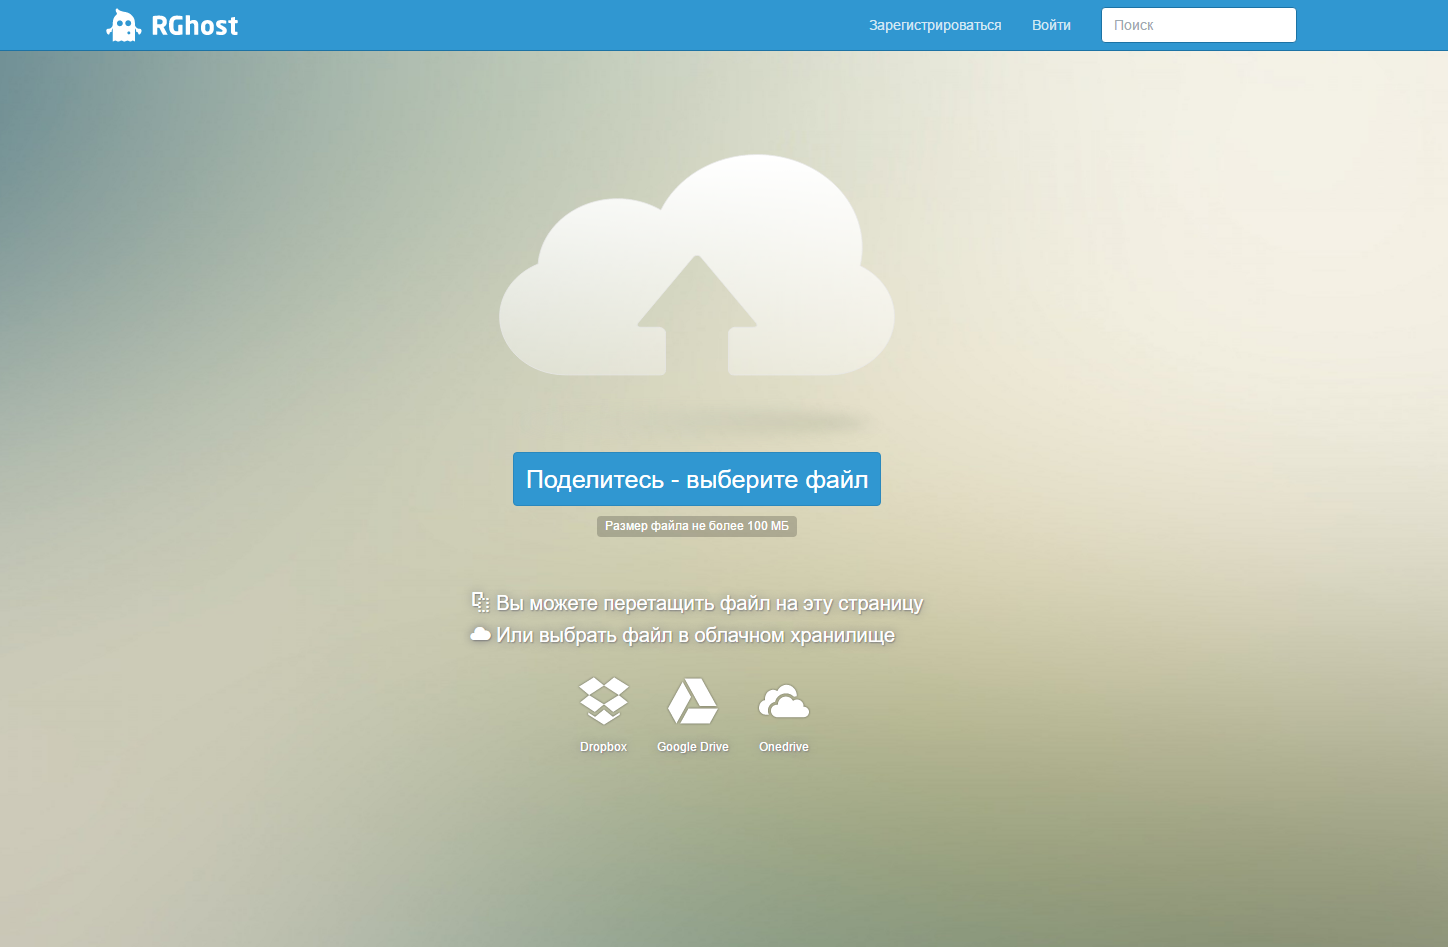
\includegraphics[scale=0.4]{rgost.png}  
    \caption{ Главная страница сервиса по обмену файлами RGhost. }
    \label{fig:rghost}
\end{figure}

Файловый хостинг «RGhost» (рисунок ~\ref{fig:rghost}) предназначен для хранения и обмена файлами между пользователями.

Данный сервис предоставляет пользователям возможность загружать не ограниченное количество файлов по суммарному объему, но размер каждого загруженного файла должен быть в пределах 50 мегабайт. Время жизни ссылок не файлы не ограничивается, но количество запросов по ссылке не должно превышать более 30 в минуту, а также данный сервис не ограничивает скорость скачивания файлов. 

Пользователям доступен следующий функционал:
\begin{itemize}
  \item неограниченый суммарный объем загруженных файлов;
  \item максимальный размер загружаемого файла - 50 мегабайт;
  \item создание бекапов меданных файла;
  \item установка пароля на файл;
  \item функция поиска;
  \item управление файлами онлайн;
  \item создание превью файла;
\end{itemize}

Сервис поддерживает большое количество вариантов оплаты премиум-аккаунта. 

Счета выставляются и оплачиваются через систему OKPAY. Она поддерживает прием следующих платежных средств напрямую: OKPAY, VISA/MC RUB, Qiwi, SofortBanking, Fortumo, Money Polo, W1, OOOPay, Alfa Click, Sberbank, PromSvyazBank, Svyaznoy, BPay.


\subsubsection{My-Files.RU}~\\
\label{ssub:practice:itechart_characteristic:myfiles}

\begin{figure}[ht]
  \centering
  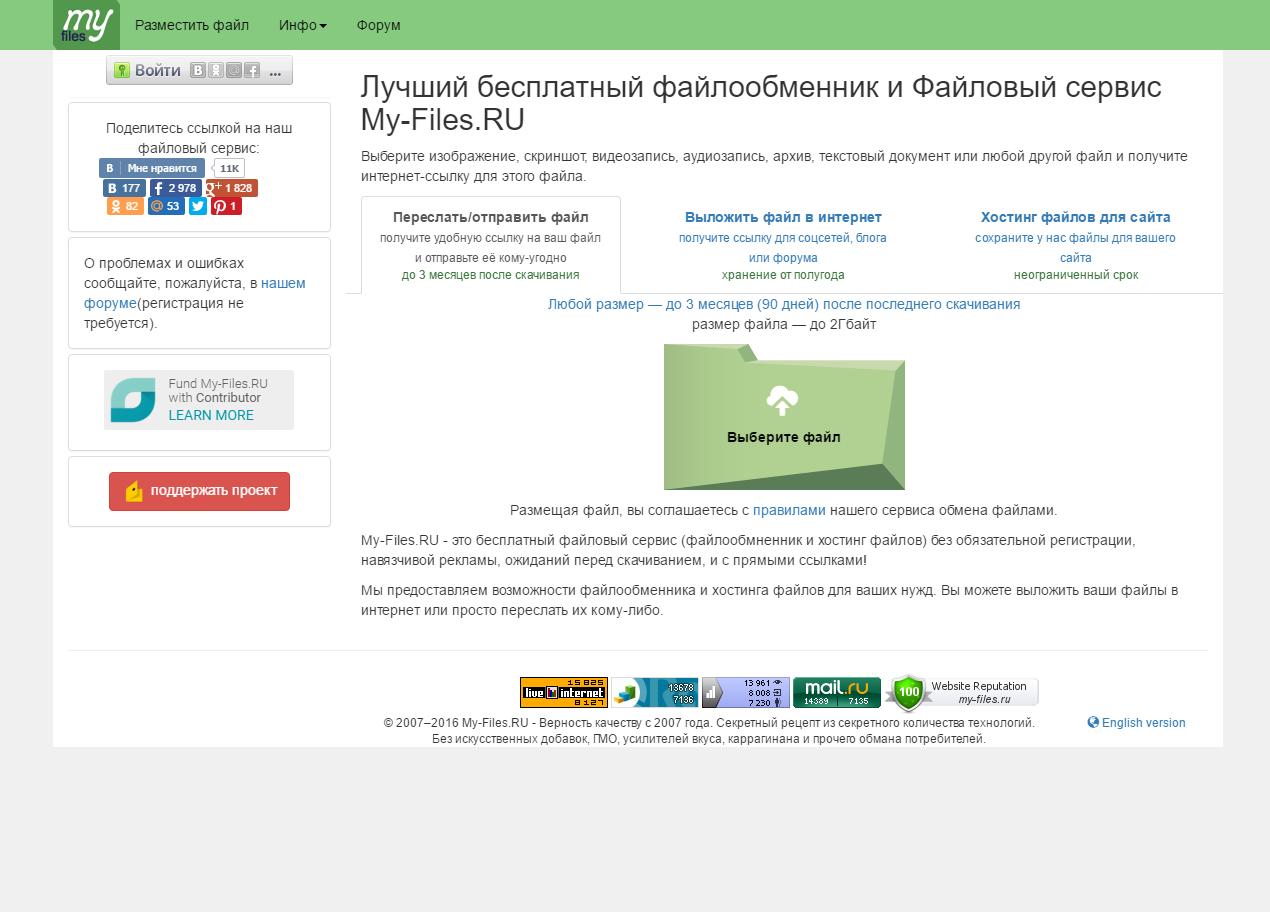
\includegraphics[scale=0.45]{my-files.png}  
    \caption{ Главная страница сервиса по обмену файлами My-Files.RU. }
    \label{fig:rghost}
\end{figure}

Сервис «My-Files.RU» позволяет загружать данные любого типа размером до 2 гигабайт, обладает форумом где можно отслеживать обновления и ошибки сервиса и способен восстанавливать удалённые файлы пользователей. 

Данный сервис позволяет генерировать ссылки на скачивание файла в желаемом формате.
Форматы представлены в виде:
\begin{itemize}
  \item короткой ссылки на файл;
  \item QR-код ссылки на файл;
  \item кодов HTML и BBCode для установки гиперссылки на файл на веб-страницах, блогах, форумах;
  \item прямой ссылки на файл.
\end{itemize} 

~\\Страница загрузки файла содержит:
\begin{itemize}
  \item информацию о файле, его размер, имя, дату размещения;
  \item для изображений - уменьшенное изображение по ширине страницы;
  \item для архивов - список содержимого архива;
  \item для исполняемых файлов - предупреждение о небезопасности файла.
\end{itemize}

Сервис «My-Files.RU» предоставляет возможность бесплатно размещать файлы в интернете для других пользователей.

Данный сервис подойдёт для таких задач как: выложить картинки, изображения, скриншоты, фото или видео; отправить большие файлы; сохранить файлы в интернете.

Кроме того, можно получить QR-код для загруженного файла, что позволит быстро загрузить файл в мобильное устройство.

\subsubsection{Файлообменник.рф}~\\
\label{ssub:practice:itechart_characteristic:fileob}

Сервис «Файлообменник.рф» - бесплатный облачный сервис для хранения файлов, куда пользователи могут загружать свои файлы, хранить их, раздавать ссылки на скачивание файлов, а также бесплатно скачивать файлы других пользователей по полученным ссылкам.

\begin{figure}[ht]
  \centering
  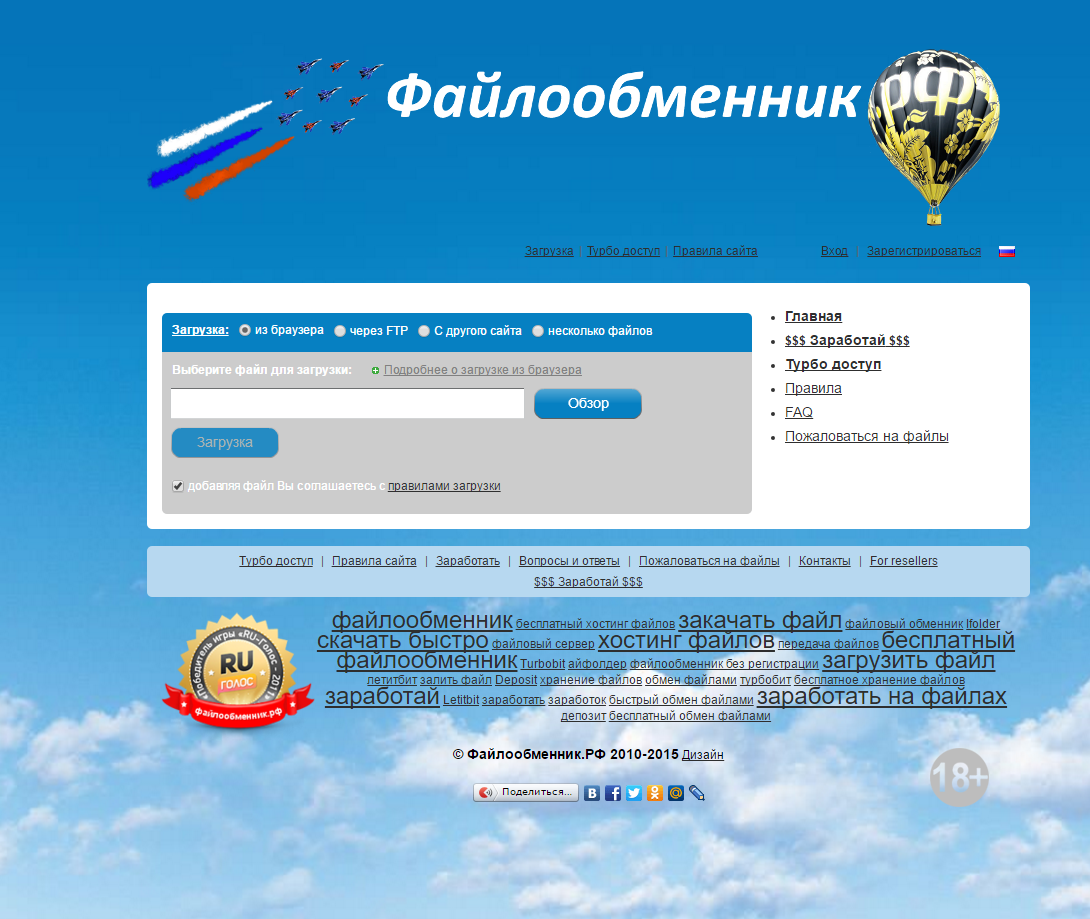
\includegraphics[scale=0.45]{fileob.png}  
    \caption{ Главная страница сервиса по обмену файлами Файлообменник.рф. }
    \label{fig:rghost}
\end{figure}

Срок хранения файлов на данном сервисе зависит от роли пользователя:
\begin{itemize}
  \item для незарегистрированных пользователей срок хранения файлов составляет 7 дней;
  \item для зарегистрированных пользователей срок хранения файлов увеличивается до 45 дней с момента его последнего скачивания;
  \item для пользователей с Турбо доступом срок хранения составляет 90 дней с момента его последнего скачивания.
\end{itemize}

~\\Максимальный размер загружаемоего файла также зависит от роли пользователя:
\begin{itemize}
  \item для незарегистрированных пользователей максимальный размер ограничен 200 Мб;
  \item для зарегистрированных пользователей максимальный размер файла 100 Гб;
  \item для пользователей с Турбо доступом максимальный размер файла также составляет 100 Гб.
\end{itemize}

Данный сервис также поддерживает программы для загрузки файлов такие как: Speedget, Download Accelerator Plus, GetRight, FlashGet и GoZilla, а так же google file download manager и т.д.

\subsubsection{Fayloobmennik.net}~\\
\label{sec:practice:itechart_characteristic:filenet}

\begin{figure}[ht]
  \centering
  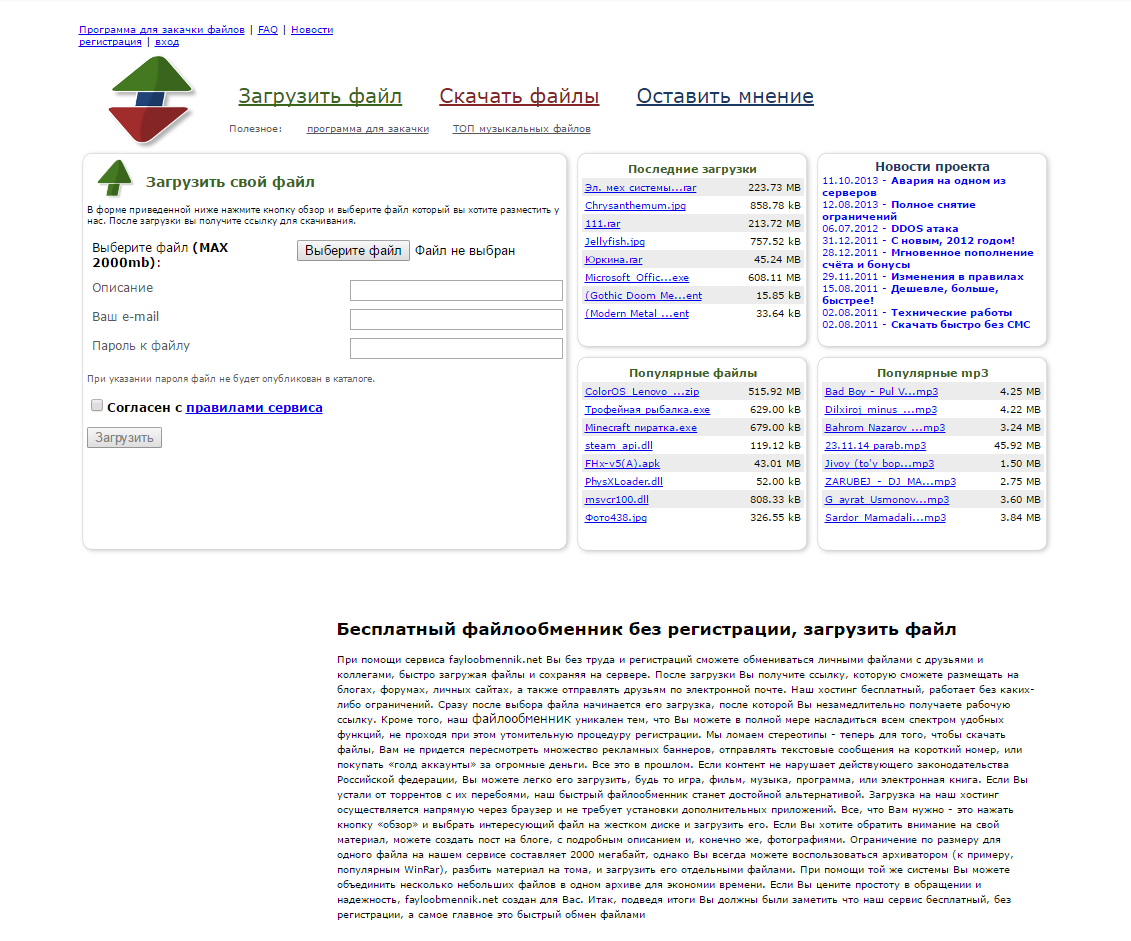
\includegraphics[scale=0.5]{failnet.png}  
    \caption{ Главная страница сервиса по обмену файлами Fayloobmennik.net. }
    \label{fig:rghost}
\end{figure}

При помощи сервиса «Fayloobmennik.net» можно без труда и регистраций обмениваться личными файлами, быстро загружая файлы и сохраняя на сервере. 

После загрузки файла на данный сервис будет предоставлена ссылка, которую можно размещать на блогах, форумах, личных сайтах, а также отправлять пользователям сети интернет по электронной почте. Данный хостинг является бесплатным и работает без каких-либо ограничений. Сразу после выбора файла начинается его загрузка, после которой незамедлительно будет сгенерирована рабочая ссылку. 

В данном сервисе есть возможность создать пост на блоге, с подробным описанием и фотографиями описывающими содержимое файла. Ограничение по размеру для одного файла на сервисе составляет 2000 мегабайт, однако можно  воспользоваться архиватором (к примеру, популярным WinRar), разбить материал на тома, и загрузить его отдельными файлами. При помощи той же системы можно объединить несколько небольших файлов в одном архиве для экономии времени.

~\\Несмотря на все преимущества рассмотренных файловых хостингов, их функциональные возможности не в полной мере соответствуют пожеланиям большинства пользователей подобных сервисов, так как требуют покупки премиум аккаунта для повышения уровня качества обслуживания, демонстрируют нежелательную рекламу во время загрузки файлов, тем самым загружая канал лишним трафиком, а также не имеют функционала ограничения доступа к файлу определенному кругу лиц. А также все эти сервисы не предоставляют должного уровня безопасности, который требуется при обмене файлами в корпоративной сети.


\subsection{Поставновка задачи}
\label{sec:practice:itechart_characteristic:zadacha}

Проанализировав основные функции, а так же все достоинства и недостатки существующих веб-приложений для обмена файлами, можно выдвинуть следующие требования к разрабатываемому веб-приложению:
\begin{itemize}
  \item  регистрация и авторизация пользователя;
  \item  загрузка и хранение файлов;
  \item  формирование ссылок на скачивание файла;
  \item  ограничение доступа к загруженным файлам;
  \item  ограничение скорости на скачивание файлов;
  \item  просмотр информации о загруженном файле
  \item  комментирование информации о файле;
  \item  поиск файлов;
  \item  управление личным аккаунтом.
\end{itemize}

Входные данные : http-запрос со стартовой строкой, заголовками и телом сообщения.

Выходные данные : http-ответ с запрашиваемой информацией или содержимым файла в теле сообщения.

Средой эксплуатации должен являться веб-сервер, поддерживающий следующие технологии:
\begin{itemize}
  \item .Net 4.5;
  \item MSSQL Server 2012;
  \item IIS 8.
\end{itemize}
